%! TeX program = lualatex

\documentclass[a4paper,14pt,final]{extarticle}
\usepackage{polyglossia} % Поддержка многоязычности (fontspec подгружается автоматически)

\setmainlanguage[babelshorthands=true]{russian} % Язык по-умолчанию русский с поддержкой приятных команд пакета babel
\PolyglossiaSetup{russian}{hyphenmins={3,3},indentfirst=true}
\setotherlanguage{english} % Дополнительный язык = английский (в американской вариации по-умолчанию)
\setmonofont{CMU Typewriter Text} % моноширинный шрифт

%\setmainfont{PT Serif}
%\usepackage{polyglossia} 

%\setdefaultlanguage{russian} 

\usepackage{OldStandard}
%\setmainfont{Times New Roman}%[Scale=0.98]
\usepackage{lualatex-math}
\usepackage{amsmath,amsthm,amssymb,amsfonts}
%
%\usepackage[math-style=ISO]{unicode-math}
%\setmathfont{Asana Math}
% \defaultfontfeatures{Scale=MatchLowercase} 
%\setmathfont{Latin Modern Math}[version=lm]


\usepackage{xfrac}
%\usepackage[T1,T2A]{fontenc}
%\usepackage[utf8]{inputenx} %% ваша любимая кодировка здесь
%\usepackage[english,russian]{babel} %% это необходимо для включения переносов
\usepackage[dvipsnames]{xcolor}
\usepackage{float}
\usepackage{graphicx}
\graphicspath{{fig/}}
%\usepackage{verbatim}
\usepackage{listings}
\usepackage{textcomp}
\usepackage{multirow,makecell}                      % Улучшенное форматирование таблиц
\usepackage[final, babel,protrusion=true, expansion=true]{microtype}
\pdfprotrudechars=2
\pdfadjustspacing=2
\newfontfeature{Microtype}{protrusion=default;expansion=default;}
\directlua{fonts.protrusions.setups.default.factor=.5}

\usepackage{epstopdf}
\usepackage{standalone}
\usepackage{pgfplots}
\usepackage{pdfpages}
\usepackage{pdfsync}
\usepackage{etoolbox}
\pgfplotsset{compat=newest}
\usepackage{subcaption}
%\usepackage{SIunits}
\usepackage{tikz}
\usepackage{needspace}
%\usepackage{subfig}
\usepackage{tabu, tabulary}
\usepackage{float}
\usepackage{luacode}
\usepackage{sidecap}
\usepackage{caption}
%\usepackage{filecontents} 
\usepackage{csquotes}
\usepackage{multicol}
%\usepackage{esvect} % вектор  
\usepackage{fancyvrb}
\usepackage[raggedright]{titlesec}  % запрет переносов в названиях секций
\usepackage{xpatch}
\usepackage{ifdraft}
\usepackage[obeyDraft]{todonotes}
\definecolor{spot}{rgb}{0,0.2,0.6}
\usepackage[
	parentracker=true,
	backend=biber,
	hyperref=auto,
	natbib=true,
	language=auto,
	autolang=other,
	citestyle=gost-numeric,
	defernumbers=true,
	bibstyle=gost-numeric
	%  sorting=none
]{biblatex}
%\addbibresource{bib/bibliography.bib}  
%\addbibresource[location=remote]{http://localhost:23119/better-bibtex/collection?/1/school.biblatex}            

\addbibresource{test1.bib}

\usepackage{standalone}
\usetikzlibrary{shapes.geometric}
\usetikzlibrary{matrix,calc}
\usepgfplotslibrary{polar}
%\input{compass}  

\usepackage{disser}
\usepackage{xfp}
\usepackage[unicode,colorlinks,allcolors=spot,breaklinks=true,bookmarksopen=true,pdfstartview=FitH]{hyperref}

%\usepackage[All]{lua-typo}


%\usepackage{background}
%\usepackage{gitinfo2}

\renewcommand\thesubfigure{\asbuk{subfigure}}

%\usepackage{sectsty}
%\allsectionsfont{\raggedright}

%\ifdraft{% Если включен режим черновика (отображение и рендер рисунков выключается)
%    \usetikzlibrary{external}\tikzexternalize[prefix=build/] % выносит графики тикза в отдельные файлы что позволяет подключать их как внешние пдф без рендера
%\pgfkeys{/pgf/images/include external/.code=\includegraphics{#1}} % в режиме черновика картинки занимают правильный размер

%\microtypesetup{draft=true}

%}{} 



\NewExpandableDocumentCommand{\getlengthnumber}{O{pt}m}{%
	% #1 (optional, default pt), #2 = length
	\fpeval{ceil((#2)/(1#1),2)}%
}


%\clubpenalty=10000      % Запрещаем разрыв страницы после первой строки абзаца
%\widowpenalty=10000     % Запрещаем разрыв страницы после последней строки абзаца
%\brokenpenalty=10000     % Ограничение на разрыв страницы, если строка заканчивается переносом
\usepackage{lua-widow-control}
%\usepackage{titlesec}
%\usepackage{titletoc}
%\titleformat{\tableofcontents}{\normalfont\bfseries}{\thetableofcontents}{0em}{}
%\titlespacing*{\tableofcontents}{0pt}{30pt}{30pt}
%\titlespacing*{\chapter}{0pt}{30pt}{30pt}
%\titlespacing*{\section}{\parindent}{*1}{*1}
%\titlespacing*{\subsection}{\parindent}{*3}{*3}
%\titlespacing*{\subsubsection}{\parindent}{*3}{*3}


%%% Переопределение именований %%%
%\renewcommand{\contentsname}{Оглавление} % (ГОСТ Р 7.0.11-2011, 4)
\addto\captionsrussian{\def\figurename{{Рисунок}}}
% (ГОСТ Р 7.0.11-2011, 5.3.9)
%\renewcommand{\tablename}{Таблица} % (ГОСТ Р 7.0.11-2011, 5.3.10)
%\addto\captionsrussian{\def\listfigurename{{\cyr\CYRS\cyrp\cyri\cyrs\cyro\cyro\cyrk~\cyrr\ciri\cyrs\cyru\cyrn\cyrk\cyro\cyrv}}}
%\renewcommand*{\listfigurename}{Список рисунков}
%\renewcommand{\listtablename}{Список таблиц}

\addto\captionsrussian{\renewcommand\listfigurename{Список рисунков}}

%\renewcommand{\contentsname}{Оглавление} % (ГОСТ Р 7.0.11-2011, 4)

%\renewcommand{\tablename}{Таблица} % (ГОСТ Р 7.0.11-2011, 5.3.10)
%\renewcommand{\listfigurename}{Список рисунков}
%\renewcommand{\listtablename}{Список таблиц}


%
% Russian sources first  
\DeclareSourcemap{
\maps[datatype=biblatex]{
\map{
  \step[fieldset=langid, fieldvalue={tempruorder}]
}
\map[overwrite]{
  \step[fieldsource=langid, match=russian, final]
  \step[fieldsource=presort, match=\regexp{(.+)}, replace=\regexp{aa$1}]  %$
}
\map{
  \step[fieldsource=langid, match=russian, final]
  \step[fieldset=presort, fieldvalue={az}]
}
\map[overwrite]{
  \step[fieldsource=langid, notmatch=russian, final]
  \step[fieldsource=presort, match=\regexp{(.+)}, replace=\regexp{za$1}]  %$
}
\map{
  \step[fieldsource=langid, notmatch=russian, final]
}
\map{
  \step[fieldsource=langid, match={tempruorder}, final]
  \step[fieldset=langid, null]
}
}
}




%\makeatletter 
%\renewcommand*\l@section{\@dottedtocline{1}{1.5em}{2.3em}}
%\makeatother

% точки для секций в содержании
\usepackage{tocloft}
\renewcommand\cftsecfont{\mdseries} % шрифт не жирный для заголовков
\renewcommand\cftsecpagefont{\mdseries} % шрифт не жирный для номеров страниц

\renewcommand{\cftsecaftersnum}{.}% точки после номера
\renewcommand{\cftsecleader}{\cftdotfill{\cftdotsep}} % точки до страницы
\setlength{\cftbeforesecskip}{0pt} % межстрочное расстояние для содержания




% для вертикального центрирования ячеек в tabulary
\def\zz{\ifx\[$\else\aftergroup\zzz\fi}
%$ \] % <-- чиним подсветку синтаксиса в некоторых редакторах
\def\zzz{\setbox0\lastbox
\dimen0\dimexpr\extrarowheight + \ht0-\dp0\relax
\setbox0\hbox{\raise-.5\dimen0\box0}%
\ht0=\dimexpr\ht0+\extrarowheight\relax
\dp0=\dimexpr\dp0+\extrarowheight\relax 
\box0
}

\lstdefinelanguage{Renhanced}%
{keywords={abbreviate,abline,abs,acos,acosh,action,add1,add,%
        aggregate,alias,Alias,alist,all,anova,any,aov,aperm,append,apply,%
        approx,approxfun,apropos,Arg,args,array,arrows,as,asin,asinh,%
        atan,atan2,atanh,attach,attr,attributes,autoload,autoloader,ave,%
        axis,backsolve,barplot,basename,besselI,besselJ,besselK,besselY,%
        beta,binomial,body,box,boxplot,break,browser,bug,builtins,bxp,by,%
        c,C,call,Call,case,cat,category,cbind,ceiling,character,char,%
        charmatch,check,chol,chol2inv,choose,chull,class,close,cm,codes,%
        coef,coefficients,co,col,colnames,colors,colours,commandArgs,%
        comment,complete,complex,conflicts,Conj,contents,contour,%
        contrasts,contr,control,helmert,contrib,convolve,cooks,coords,%
        distance,coplot,cor,cos,cosh,count,fields,cov,covratio,wt,CRAN,%
        create,crossprod,cummax,cummin,cumprod,cumsum,curve,cut,cycle,D,%
        data,dataentry,date,dbeta,dbinom,dcauchy,dchisq,de,debug,%
        debugger,Defunct,default,delay,delete,deltat,demo,de,density,%
        deparse,dependencies,Deprecated,deriv,description,detach,%
        dev2bitmap,dev,cur,deviance,off,prev,,dexp,df,dfbetas,dffits,%
        dgamma,dgeom,dget,dhyper,diag,diff,digamma,dim,dimnames,dir,%
        dirname,dlnorm,dlogis,dnbinom,dnchisq,dnorm,do,dotplot,double,%
        download,dpois,dput,drop,drop1,dsignrank,dt,dummy,dump,dunif,%
        duplicated,dweibull,dwilcox,dyn,edit,eff,effects,eigen,else,%
        emacs,end,environment,env,erase,eval,equal,evalq,example,exists,%
        exit,exp,expand,expression,External,extract,extractAIC,factor,%
        fail,family,fft,file,filled,find,fitted,fivenum,fix,floor,for,%
        For,formals,format,formatC,formula,Fortran,forwardsolve,frame,%
        frequency,ftable,ftable2table,function,gamma,Gamma,gammaCody,%
        gaussian,gc,gcinfo,gctorture,get,getenv,geterrmessage,getOption,%
        getwd,gl,glm,globalenv,gnome,GNOME,graphics,gray,grep,grey,grid,%
        gsub,hasTsp,hat,heat,help,hist,home,hsv,httpclient,I,identify,if,%
        ifelse,Im,image,\%in\%,index,influence,measures,inherits,install,%
        installed,integer,interaction,interactive,Internal,intersect,%
        inverse,invisible,IQR,is,jitter,kappa,kronecker,labels,lapply,%
        layout,lbeta,lchoose,lcm,legend,length,levels,lgamma,library,%
        licence,license,lines,list,lm,load,local,locator,log,log10,log1p,%
        log2,logical,loglin,lower,lowess,ls,lsfit,lsf,ls,machine,Machine,%
        mad,mahalanobis,make,link,margin,match,Math,matlines,mat,matplot,%
        matpoints,matrix,max,mean,median,memory,menu,merge,methods,min,%
        missing,Mod,mode,model,response,mosaicplot,mtext,mvfft,na,nan,%
        names,omit,nargs,nchar,ncol,NCOL,new,next,NextMethod,nextn,%
        nlevels,nlm,noquote,NotYetImplemented,NotYetUsed,nrow,NROW,null,%
        numeric,\%o\%,objects,offset,old,on,Ops,optim,optimise,optimize,%
        options,or,order,ordered,outer,package,packages,page,pairlist,%
        pairs,palette,panel,par,parent,parse,paste,path,pbeta,pbinom,%
        pcauchy,pchisq,pentagamma,persp,pexp,pf,pgamma,pgeom,phyper,pico,%
        pictex,piechart,Platform,plnorm,plogis,plot,pmatch,pmax,pmin,%
        pnbinom,pnchisq,pnorm,points,poisson,poly,polygon,polyroot,pos,%
        postscript,power,ppoints,ppois,predict,preplot,pretty,Primitive,%
        print,prmatrix,proc,prod,profile,proj,prompt,prop,provide,%
        psignrank,ps,pt,ptukey,punif,pweibull,pwilcox,q,qbeta,qbinom,%
        qcauchy,qchisq,qexp,qf,qgamma,qgeom,qhyper,qlnorm,qlogis,qnbinom,%
        qnchisq,qnorm,qpois,qqline,qqnorm,qqplot,qr,Q,qty,qy,qsignrank,%
        qt,qtukey,quantile,quasi,quit,qunif,quote,qweibull,qwilcox,%
        rainbow,range,rank,rbeta,rbind,rbinom,rcauchy,rchisq,Re,read,csv,%
        csv2,fwf,readline,socket,real,Recall,rect,reformulate,regexpr,%
        relevel,remove,rep,repeat,replace,replications,report,require,%
        resid,residuals,restart,return,rev,rexp,rf,rgamma,rgb,rgeom,R,%
        rhyper,rle,rlnorm,rlogis,rm,rnbinom,RNGkind,rnorm,round,row,%
        rownames,rowsum,rpois,rsignrank,rstandard,rstudent,rt,rug,runif,%
        rweibull,rwilcox,sample,sapply,save,scale,scan,scan,screen,sd,se,%
        search,searchpaths,segments,seq,sequence,setdiff,setequal,set,%
        setwd,show,sign,signif,sin,single,sinh,sink,solve,sort,source,%
        spline,splinefun,split,sqrt,stars,start,stat,stem,step,stop,%
        storage,strstrheight,stripplot,strsplit,structure,strwidth,sub,%
        subset,substitute,substr,substring,sum,summary,sunflowerplot,svd,%
        sweep,switch,symbol,symbols,symnum,sys,status,system,t,table,%
        tabulate,tan,tanh,tapply,tempfile,terms,terrain,tetragamma,text,%
        time,title,topo,trace,traceback,transform,tri,trigamma,trunc,try,%
        ts,tsp,typeof,unclass,undebug,undoc,union,unique,uniroot,unix,%
        unlink,unlist,unname,untrace,update,upper,url,UseMethod,var,%
        variable,vector,Version,vi,warning,warnings,weighted,weights,%
        which,while,window,write,\%x\%,x11,X11,xedit,xemacs,xinch,xor,%
        xpdrows,xy,xyinch,yinch,zapsmall,zip},%
    otherkeywords={!,!=,~,$,*,\%,\&,\%/\%,\%*\%,\%\%,<-,<<-},%$
    alsoother={._$},%$
    sensitive,%
    morecomment=[l]\#,%
    morestring=[d]",%
    morestring=[d]'% 2001 Robert Denham
}%


%решаем проблему с кириллицей в комментариях (в pdflatex) https://tex.stackexchange.com/a/103712
\lstset{extendedchars=true,keepspaces=true,literate={Ö}{{\"O}}1
    {Ä}{{\"A}}1
    {Ü}{{\"U}}1
    {ß}{{\ss}}1
    {ü}{{\"u}}1
    {ä}{{\"a}}1
    {ö}{{\"o}}1
    {~}{{\textasciitilde}}1
    {а}{{\selectfont\char224}}1
    {б}{{\selectfont\char225}}1
    {в}{{\selectfont\char226}}1
    {г}{{\selectfont\char227}}1
    {д}{{\selectfont\char228}}1
    {е}{{\selectfont\char229}}1
    {ё}{{\"e}}1
    {ж}{{\selectfont\char230}}1
    {з}{{\selectfont\char231}}1
    {и}{{\selectfont\char232}}1
    {й}{{\selectfont\char233}}1
    {к}{{\selectfont\char234}}1
    {л}{{\selectfont\char235}}1
    {м}{{\selectfont\char236}}1
    {н}{{\selectfont\char237}}1
    {о}{{\selectfont\char238}}1
    {п}{{\selectfont\char239}}1
    {р}{{\selectfont\char240}}1
    {с}{{\selectfont\char241}}1
    {т}{{\selectfont\char242}}1
    {у}{{\selectfont\char243}}1
    {ф}{{\selectfont\char244}}1
    {х}{{\selectfont\char245}}1
    {ц}{{\selectfont\char246}}1
    {ч}{{\selectfont\char247}}1
    {ш}{{\selectfont\char248}}1
    {щ}{{\selectfont\char249}}1
    {ъ}{{\selectfont\char250}}1
    {ы}{{\selectfont\char251}}1
    {ь}{{\selectfont\char252}}1
    {э}{{\selectfont\char253}}1
    {ю}{{\selectfont\char254}}1
    {я}{{\selectfont\char255}}1
    {А}{{\selectfont\char192}}1
    {Б}{{\selectfont\char193}}1
    {В}{{\selectfont\char194}}1
    {Г}{{\selectfont\char195}}1
    {Д}{{\selectfont\char196}}1
    {Е}{{\selectfont\char197}}1
    {Ё}{{\"E}}1
    {Ж}{{\selectfont\char198}}1
    {З}{{\selectfont\char199}}1
    {И}{{\selectfont\char200}}1
    {Й}{{\selectfont\char201}}1
    {К}{{\selectfont\char202}}1
    {Л}{{\selectfont\char203}}1
    {М}{{\selectfont\char204}}1
    {Н}{{\selectfont\char205}}1
    {О}{{\selectfont\char206}}1
    {П}{{\selectfont\char207}}1
    {Р}{{\selectfont\char208}}1
    {С}{{\selectfont\char209}}1
    {Т}{{\selectfont\char210}}1
    {У}{{\selectfont\char211}}1
    {Ф}{{\selectfont\char212}}1
    {Х}{{\selectfont\char213}}1
    {Ц}{{\selectfont\char214}}1
    {Ч}{{\selectfont\char215}}1
    {Ш}{{\selectfont\char216}}1
    {Щ}{{\selectfont\char217}}1
    {Ъ}{{\selectfont\char218}}1
    {Ы}{{\selectfont\char219}}1
    {Ь}{{\selectfont\char220}}1
    {Э}{{\selectfont\char221}}1
    {Ю}{{\selectfont\char222}}1
    {Я}{{\selectfont\char223}}1
    {і}{{\selectfont\char105}}1
    {ї}{{\selectfont\char168}}1
    {є}{{\selectfont\char185}}1
    {ґ}{{\selectfont\char160}}1
    {І}{{\selectfont\char73}}1
    {Ї}{{\selectfont\char136}}1
    {Є}{{\selectfont\char153}}1
    {Ґ}{{\selectfont\char128}}1
}

% Ширина текста минус ширина надписи 999
\newlength{\twless}
\newlength{\lmarg}
\setlength{\lmarg}{\widthof{999}}   % ширина надписи 999
\setlength{\twless}{\textwidth-\lmarg}



\lstset{ %
%    language=R,                     %  Язык указать здесь, если во всех листингах преимущественно один язык, в результате часть настроек может пойти только для этого языка
    numbers=left,                   % where to put the line-numbers
    numberstyle=\fontsize{12pt}{14pt}\selectfont\color{Gray},  % the style that is used for the line-numbers
    firstnumber=1,                  % в этой и следующей строках задаётся поведение нумерации 5, 10, 15...
    stepnumber=1,                   % the step between two line-numbers. If it's 1, each line will be numbered
    numbersep=5pt,                  % how far the line-numbers are from the code
    backgroundcolor=\color{white},  % choose the background color. You must add \usepackage{color}
    showspaces=false,               % show spaces adding particular underscores
    showstringspaces=false,         % underline spaces within strings
    showtabs=false,                 % show tabs within strings adding particular underscores
    frame=leftline,                 % adds a frame of different types around the code
    rulecolor=\color{black},        % if not set, the frame-color may be changed on line-breaks within not-black text (e.g. commens (green here))
    tabsize=2,                      % sets default tabsize to 2 spaces
    captionpos=t,                   % sets the caption-position to top
    breaklines=true,                % sets automatic line breaking
    breakatwhitespace=false,        % sets if automatic breaks should only happen at whitespace
    %title=\lstname,                 % show the filename of files included with \lstinputlisting;
    % also try caption instead of title
    basicstyle=\fontsize{12pt}{14pt}\selectfont\ttfamily,% the size of the fonts that are used for the code
    keywordstyle=\color{blue},      % keyword style
    commentstyle=\color{ForestGreen}\emph,% comment style
    stringstyle=\color{Mahogany},   % string literal style
    escapeinside={\%*}{*)},         % if you want to add a comment within your code
    morekeywords={*,...},           % if you want to add more keywords to the set
    inputencoding=utf8,             % кодировка кода
    xleftmargin={\lmarg},           % Чтобы весь код и полоска с номерами строк была смещена влево, так чтобы цифры не вылезали за пределы текста слева
} 


\makeatletter
\DeclareRobustCommand{\getlstname}{%
 \begingroup
  % \lstname seems to change hyphens into \textendash
  \def\textendash{-}%
  \filename@parse{\lstname}%
  \texttt{\filename@base.\filename@ext}%
 \endgroup
}
\makeatother



%http://tex.stackexchange.com/questions/26872/smaller-frame-with-listings
% Окружение, чтобы листинг был компактнее обведен рамкой, если она задается, а не на всю ширину текста
\makeatletter
\newenvironment{SmallListing}[1][]
{\lstset{#1}\VerbatimEnvironment\begin{VerbatimOut}{VerbEnv.tmp}}
{\end{VerbatimOut}\settowidth\@tempdima{%
        \lstinputlisting{VerbEnv.tmp}}
    \minipage{\@tempdima}\lstinputlisting{VerbEnv.tmp}\endminipage}    
\makeatother


\DefineVerbatimEnvironment% с шрифтом 12 пт
{Verb}{Verbatim}
{fontsize=\fontsize{12pt}{14pt}\selectfont}

%\newfloat[section]{ListingEnv}{lol}{Листинг}

\renewcommand{\lstlistingname}{Листинг}

%Общие счётчики окружений листингов
%http://tex.stackexchange.com/questions/145546/how-to-make-figure-and-listing-share-their-counter
% Если смешивать плавающие и не плавающие окружения, то могут быть проблемы с нумерацией
\makeatletter
\AtBeginDocument{%
    \let\c@ListingEnv\c@lstlisting
    \let\theListingEnv\thelstlisting
    \let\ftype@lstlisting\ftype@ListingEnv % give the floats the same precedence
}
\makeatother

% значок С++ — используйте команду \cpp
\newcommand{\cpp}{%
    C\nolinebreak\hspace{-.05em}%
    \raisebox{.2ex}{+}\nolinebreak\hspace{-.10em}%
    \raisebox{.2ex}{+}%
}

% Замена URL на стрелку 
%\usepackage{bbding}
%\renewcommand{\url}[1]{\href{#1}{\ArrowBoldUpRight}}
%%%%%%%%%%%%%%%%%%%
%URL  не конвертируются в %D1
\DeclareFieldFormat{url}{%
	\mkbibacro{URL}\addcolon\space
	\href{#1}{\nolinkurl{\thefield{urlraw}}}}



\begin{document}
%\IfFileExists{title.pdf}{\includepdf[pages=-]{title}}{}



%\large
%\usefont{T2A}{ftm}{m}{} %%% Использование шрифтов Т2 для возможности копировать екст из PDF-файлов.


%===================Параметры Страницы (поля,ширина,высота)=================-=====================
%\headheight=0mm       %размер места отводимого под колонтитул
%\headsep=0mm          %отступ между колонтитулом и основным текстом
%\oddsidemargin=1mm    %левое поле
%\topmargin=-10mm    %верхнее поле
%\textheight=247mm     %высота текста
%\textwidth=160mm      %ширина текста
%\setcounter{page}{3}
%\renewcommand{\baselinestretch}{1.5}.
%\setcounter{chapter}{1} 

% 
%


\title{РЕКОМЕНДАЦИИ ПО ОФОРМЛЕНИЮ ПОЯСНИТЕЛЬНЫХ ЗАПИСОК}

\author{Бондаренко Михаил Анатольевич}
\date{\it \href{mailto:bondarenkoma@mail.ru}{bondarenkoma@mail.ru}}
\maketitle
%\noindent\hrulefill
\microtypesetup{protrusion=false} % disables protrusion locally in the document
\tableofcontents % prints Table of Contents
\microtypesetup{protrusion=true} % enables protrusion

%\clearpage

% !TeX root=work-template.tex
  
\section{Введение}
Как и любой другой документ, пояснительная записка должна четко и ясно доносить до читателя идею автора, так же, как и соответствовать определенным требованиям перечисленным в данном документе. Набор пояснительной записки с учетом установленных правил удобнее всего осуществлять в текстовых редакторах Word, Writer, \LaTeX и других.

  
\section{Содержание пояснительной записки}
В работе должны быть четко выделены и обозначены следующие пункты в порядке их очереди в пояснительной записке:
\begin{enumerate}
    \item Титульный лист. Необходимо указать Ваше ФИО и научного руководителя, название проекта, и организацию при которой проект был разработан. В каждом конкретном случае варианты оформления могут отличаться.
    \item Содержание. 
    \item Введение. Общее описание задачи и актуальность проблемы, не нумеруется, указывается в содержании;
    \item Постановка задачи. Описание задачи которая ставилась перед автором расписанная по пунктам;
    \item Использованные методы. Названием раздела служит название использованного вами метода или группы методов (например: Теория перколяции; Скрытые марковские модели; и т.д.), в описании раздела следуют расписать как и какой метод(ы) применялись;
    \item Тестирование. Необходимый пункт если в работе подразумевается создание модели, в этом пункте необходимо описать процедуру тестирования и какие результаты были получены, описать почему модель адекватна задаче;
    \item Результаты. Полученные результаты при проведении моделирования или симуляции если таковая была; 
    \item Выводы. Сопоставить результаты и поставленную задачу, сделать выводы о полученных результатах, указать возможное дальнейшее развитие;
    \item Список использованных источников. Указывается в содержании, но не нумеруется. Необходимо указывать автора, год, полное название книги/статьи/журнала. Оформляется по ГОСТу \cite{BibStandart2007}. 
    \item Приложения. Если в работе есть иллюстрирующий материал, тексты программ, 
    какая либо важная     для общего представления о работе информация, то она помещается в этот раздел.     Приложения нумеруются буквами кириллического алфавита (например: Приложение~А. Текст 
    программы,     Приложение~Б. Результаты для смежной задачи, и~т.д.)
\end{enumerate}

\section{Общие требования}
Оформление осуществляется по ГОСТу \cite{Standart2017}, также можно воспользоваться руководству по набору в соответствии с правилами ГОСТа\cite{rule}. Страница формата А4, цвет шрифта должен быть черным, размер шрифта - не менее 12 пт. Тип шрифта для основного текста отчета - Times New Roman, использование других шрифтов возможно только для текста программ, где применятся любой моноширинный шрифт (без засечек). Полужирный шрифт применяют только для заголовков разделов и подразделов, заголовков структурных элементов. 
\par <<Введение>> и <<Список использованных источников>> не нумеруется, но в содержании учитывается. 
\par  Отступы полей страницы составляют левое 3~см, правое 1.5~см, верхнее и нижнее 2~см. Абзацный отступ (красная строка) должен быть одинаковым по всему тексту отчета и равен 1,25~см. Страницы нумеруются снизу, по центру. Выравнивание текста по ширине. 
%\getlengthnumber[cm]{\hoffset}
\begin{figure}[H]
\centering
\def\xis{0}
\def\xie{4}
\def\yis{0}
\def\yie{6}
%
\def\xos{-2}
\def\xoe{5.5}
\def\yos{-1}
\def\yoe{7}
%
    \begin{tikzpicture}
        \draw [draw=black] (\xis,\yis)  rectangle (\xie,\yie);
        \draw [draw=black] (\xos,\yos)  rectangle (\xoe,\yoe);
        \draw[thick,<->] (\xos,3) -- (\xis,3) node[midway,above] {3см};
        \draw[thick,<->] (1,\yie) -- (1,\yoe) node[midway,right] {2см};
        \draw[thick,<->] (\xie,3) -- (\xoe,3) node[midway,above] {1.5см};
        \draw[thick,<->] (1,\yis) -- (1,\yos) node[midway,right] {2см};
    \end{tikzpicture}
    \caption{Наглядное представление отступов на листе формата А4.}
\end{figure}
\par Каждый новый раздел (Например: 7. Результаты) должен начинаться с новой страницы, однако подразделы (Например 7.1 Название подраздела) можно не переносить на новую страницу. 
\par Использование курсива допускается для обозначения объектов ({\it биология, геология, медицина, нанотехнологии, генная инженерия} и др.) и написания терминов (например, {\it iin vivo, in vitro}) и иных объектов и терминов на латыни.
\subsection{Теоремы, доказательства, определения, аксиомы и т.д.}
\par Как таковых жестких требований к оформлению такого рода объектов~нет, однако есть общепринятый вариант распространенный в технической литературе, обычно они оформляются как выносной блок с нумерацией. Пример оформления теорем:
\begin{theorem}[Теорема Коши о среднем значении] 
    Пусть $f(x)$ и $g(x)$ непрерывны на отрезке $[a,b]$ и дифференцируемы на интервале $(a,b)$...
\end{theorem}
Нумерация нужна чтобы ссылаться на ту или иную теорему в других местах работы.
    
\subsection{Формулы}
\par Формулы располагаются по центру и обязательно должны иметь номер по правой стороне страницы. Например: 
\begin{equation} 
    \iint\limits_{G} \frac{\partial Q(x,y)}{\partial x}dxdy = \int\limits_{\partial G} Q(x,y)dy.
\end{equation}  
\par После формул ставится тот знак препинания, который необходим исходя из построения фразы: если формулой заканчивается фраза -- точка, если заканчивается главное предложение -- запятая (например, перед сло­вом где, начинающим экспликацию). В системах уравнений, каждое уравнение отделяется точкой с запятой, а последнее уравнение точка или точка с запятой в зависимости от того начинаются ли дальше новое предложение или идут пояснения с текущему.
\subsubsection{Нумерация}
При наличии в тексте ссылок на формулы обычно применяют сквозную порядковую нумерацию ограниченного числа наиболее важных формул пря­мыми арабскими цифрами в круглых скобках.

Когда очередная формула является разновидностью приведенной ра­нее основной формулы, допускается нумерация формулы арабской цифрой и строчной прямой буквой русского алфавита, набираемой вплотную к цифре. Например: (37а), (37б) и т. д.

В больших работах (учебниках, монографиях, справочниках) допус­кается применение двойной порядковой нумерации по разделам (главам). В этом случае первое число нумерации соответствует номеру раздела или главы, второе — порядковому номеру формулы внутри раздела или главы. Напри­мер, 18-я по порядку формула в главе 6 нумеруется (6.18), формула 43а в раз­деле 2 нумеруется (2.43а).

Для промежуточных формул, приводимых для вывода основных фор­мул, применяют нумерацию строчными буквами русского алфавита, наби­раемыми прямым шрифтом в круглых скобках.
Порядковые номера всех формул помещают в круглых скобках у пра­вого края полосы без отточия от формулы к ее номеру.

При наборе формулы в рамку номер ее следует помещать вне рамки в правый край основной строки формулы.
Для формулы, представляющей собой дробь с горизонтальной чертой как знаком деления, номер выключается по середине основной ли­нейки.

Номер для многострочной формулы ставится против последней ее строки. При нумерации группы формул применяют фигурные скобки, охваты­вающие по высоте все формулы, с обращением острия скобки против середины этой группы в сторону порядкового номера, помещаемого в скобке против острия у правого края страницы. 

В тексте ссылку на порядковый номер следует начинать со слов фор­мула, уравнение, выражение и затем в круглых скобках указывают номер формулы. Например: в формуле (4.15) приведены...

Если ссылка на порядковый номер формулы находится внутри выра­жения, заключенного в круглые скобки, то их следует заменить на прямые скобки. Например: Удельная теплоемкость кислорода (см. уравнение (43)) увеличивается с ростом температуры.

\subsubsection{Экспликация}
В экспликацию -- расшифровку приведенных в формуле буквенных обозначений величин следует, как правило, включать все обозначения, помещенные как в левой, так и в правой части формулы.

Если перед формулой помещено обозначение единицы, приво­димое в левой части формулы, то в экспликации ее можно не приводить.

Последовательность расшифровки буквенных обозначений величин должна соответствовать последовательности расположения этих обозначений в формуле. Если правая часть формулы представляет собой дробь, то вначале поясняются обозначения величин, помещенных в числителе, а затем — в знаменателе.

После формулы перед экспликацией следует поставить запятую, затем с новой строки набрать от левого края слово где (без двоеточия после него), за ним — обозначение первой величины и его расшифровку и далее с новой строки каждое следующее обозначение и его расшифровку, выравни­вая колонку расшифровок по знаку тире. Эти знаки должны образовать вер­тикаль.

Для издания, где необходима особая компактность набора (справочники, энциклопедии и т. и.), допускается набор строк экспликации в подбор.

Если расшифровка обозначения не умещается в одной строке, то вто­рая и следующая строки расшифровки должны начинаться от нового края первого слова расшифровки первой строки. В конце каждой расшифровки рекомендуется ставить точку с занятой, а в конце последней расшифровки — точку.

Обозначения единиц физических величин в каждой расшифровке следует отделять занятой от текста расшифровки.
\needspace{5cm}
Например: 
\[
\tag{{\theequation}a}
\frac{b}{D} = \rho, 
\]
где
\begin{enumerate}
    \item [b] -- толщина стенки, м;
    \item [D] -- внутренний диаметр, м;
    \item [\rho] -- давление, Па.
\end{enumerate}

При повторении в последующих формулах обозначений величин, приведенных в предыдущих формулах, допускается повторение их расшиф­ровки, если формулы отдалены друг от друга. Можно ограничиться ссылкой на порядковый номер формулы, при которой приведена расшифровка.

\subsubsection{Перенос формул}

Если формула настолько длинна, что она не умещается в одной строке, то ее частично переносят на другую строку. В первую очередь перенос следует делать на знаках равенства и соотношения между левой и правой частями формулы, во вторую на отточии (...), зна­ках сложения и вычитания, в третью — на знаке умножения с применением косого креста (\(\times \)) в конце одной строки и в начале следующей стро­ки. Не допускаются переносы на знаке деления.

При переносе формул не допускается разделение индексов, показа­телей степени, а также выражений, относящихся к знакам логарифма, инте­грала, тригонометрических функций, суммы \( (  \sum ) \) и произведения \( (\prod)\).

Если при коротком знаменателе часть числителя дроби с горизон­тальной чертой не умещается в формате набора, рекомендуется записать чис­литель в виде многочлена в скобках и заменить горизонтальную черту косой в качестве знака деления либо привести формулу к виду, в котором единица, деленная на знаменатель, умножается на числитель. В обоих случаях раз­бивают формулу переносом на знаке плюс или минус многочлена.

Если при коротком числителе часть знаменателя в дроби с горизон­тальной чертой (знак деления) не умещается в формате набора, рекомендуется заменить горизонтальную черту косой в качестве знака деления, записав числитель и знаменатель в виде многочлена в скобках, либо заменить отдель­ные сложные элементы знаменателя упрощенными условными обозначениями, расшифрованными вслед за формулой.

Рекомендации по переносу формул в виде дроби с длинным числите­лем и длинным знаменателем аналогичны рекомендациям выше.

Если в формат набора не умещается длинное подкоренное выражение с показателем корня \(n\), его можно преобразовать путем возвышения в степень \(1/n\) подкоренного выражения.

\subsection{Рисунки, графики и изображения}
\par Помните, все графики и рисунки которые вы используете в работе должны быть ее частью. Если целью вашего проекта не является изучение жизни и личности, то не используйте обширные исторические вставки с фотографиями и биографией.
Картинки и иллюстрирующий материалы должны иметь выравнивание по центру, номер и краткое описание. 

Например:
\begin{figure}[H]
    \centering
    %\includegraphics[width=.3\textwidth]{example-grid-100x100pt}
    \includegraphics[width=.4\textwidth]{example-image-a}
    %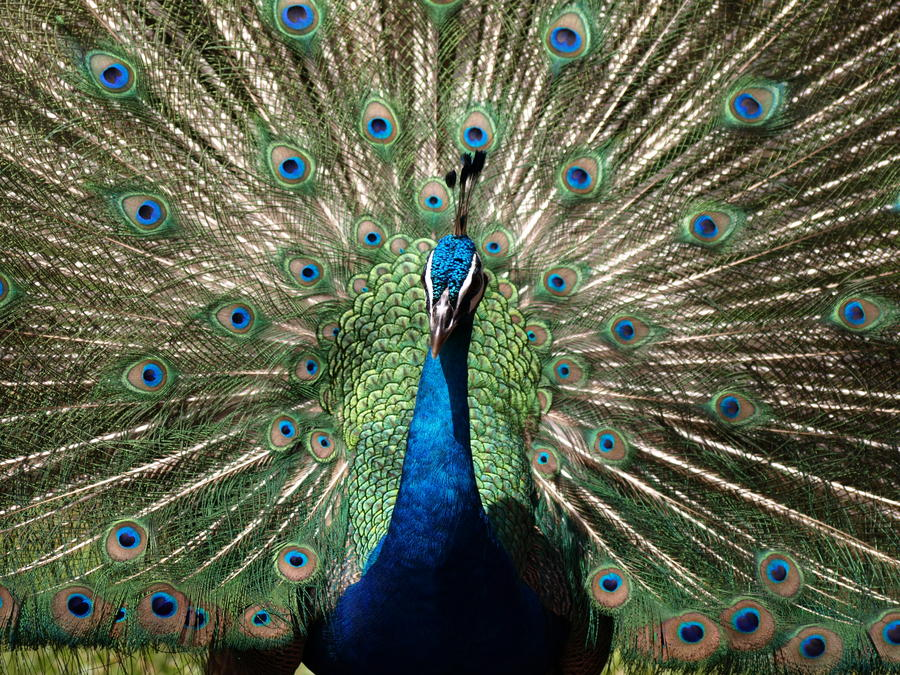
\includegraphics[width=.3\textwidth]{pics/sample_01.jpg}
    \caption{Краткое описание картинки.}
\end{figure} 
\par Если рисунок представляет собой график, то оси обязательно должны быть подписаны. Если на рисунке совмещено несколько графиков, тогда необходимо описание для каждого. Например:
 
\begin{figure}[H]
    \centering
    \begin{tikzpicture}
        \begin{axis}[axis lines=middle,samples=20,xlabel=$x$,ylabel=$y$,legend pos=south east]
        %\addplot[blue,domain=-3:1.85] {1/(x-2) +3 };
        \addplot[,black,domain=-3:3] {x*x};
        \addlegendentry{$f(x)=x^2$}

        \addplot[dashed,black,domain=-3:3] {x*5};% node [pos=0.3, below right] {$g(x)=5x$};;
        \addlegendentry{$g(x)=5x$}
        \end{axis}
        \end{tikzpicture}
        \caption{Пример оформления графика.}
\end{figure}
 
\par Массивы картинок можно объединять под одним номером, но в этом случае у каждой картинки должны быть 
собственные подпись и буквенный номер. 
Например:~%
\begin{figure}[H]
    \centering
    \begin{subfigure}[t]{0.45\textwidth}
        \centering
        \includegraphics[width=0.8\textwidth]{example-image-a}
        \caption{Подпись к рисунку.}
    \end{subfigure}
    \begin{subfigure}[t]{0.45\textwidth}
        \centering
        \includegraphics[width=0.8\textwidth]{example-image-b}
        \caption{Подпись к рисунку.}
    \end{subfigure}
    \caption{Подпись к группе рисунков.}
\end{figure}
\subsection{Таблицы}
\par Таблицы располагаются по центру, вместе с номером и подписью, которые находиться над таблицей. Например:~
\begin{table}[H]
    \centering
    \caption{\label{table}Краткое описание таблицы.}
    \begin{tabular}{|c|c|}
        \hline
        \bf{Название колонки 1} & \bf{Название колонки 2}  \\
        \hline
        Данные 1 & Данные 2 \\
        \hline
        Данные 3 & Данные 4 \\
        \hline
       \end{tabular}
\end{table}  
\par Длинные таблицы должны повторять <<шапку>> таблицы на каждой странице.


\section{Библиографические ссылки}
В работе необходимо указывать библиографические ссылки на используемые источники. Нумерация их в разделе <<Список использованных источников>> может быть как в порядке их использования в работе, так и в алфавитном. 
\par При указании ссылки, номер используемого источника указывается в квадратных скобках (например: При составлении данного документа использовались правила ГОСТ \cite{Standart2017}). Пример создания библиографии в редакторе Word \cite{wordexpample}. 
\par URL на ресурсы и источники данных в разделе <<Список использованных источников>> следует также вставлять либо целиком, если работа предназначена для распечатывания, либо заменять на символ ссылки.

\section{Презентация}
При оформлении презентации, стенда или другого способа донести информацию до аудитории, по мимо общих требований, необходимо учитывать следующее:
\paragraph{Содержание презентации.} Структура презентации и в пояснительной записки должна быть одинаковой. Не используйте большое количество текста на слайде. Слайды состоящие целиком из текста плохо воспринимаются, постарайтесь проговорить текст, а вместо него вставить информативную и напрямую относящуюся к тексту картинку. 
\paragraph{Фон и цвет.} Используйте только светлый фон, в идеале белый, и черный цвет шрифта. Допускается оформление краев слайдов, но не более 5\% от общей площади слайда. 
\paragraph{Шрифт.} Для создания презентации рекомендуют использовать шрифты Arial или Times New 
    Roman. Это обусловлено тем, что эти шрифты есть на любом компьютере. 
    Если же использовать редкий шрифт, то при использовании презентации на неизвестном 
    компьютере, в котором нет используемого шрифта, на экране будут отображаться квадратики или
     непонятные символы. 
     Печатайте информацию достаточно крупным кеглем без использования CapsLock. Если вам 
     нужно выделить слово или выражение, используйте лучше полужирный шрифт.
\paragraph{Графика.} С ее помощью вы можете проиллюстрировать информацию, которую хотите представить комиссии на защите. При использовании диаграмм или графиков обязательно указывайте на слайдах внизу расшифровку сокращений, и подписи к осям координатным. При этом каждая иллюстрация должна сопровождаться подписью, пример можно видеть на рисунке~\ref{pic-pres-graph}. 
\paragraph{Таблицы.} Программы для презентаций, как правило, не любят таблиц. Если вы хотите поместить чрезвычайно важную информацию в форме таблицы, вставьте ее в слайд как картинку. Если это невозможно ввиду разнородности информации в таблице, постарайтесь уместить таблицу на одном слайде, выделив важную информацию жирным или полужирным.
\paragraph{Анимация.} Анимацию не следует использовать, если вы, не выпускник режиссерских специальностей. Исчезайте, всплывание, растворение надписей оказывает впечатление несерьезности, что вовсе ни к чему при защите проектной или дипломной работы.
\paragraph{Звуковые эффекты.} Не используйте звуковые эффекты при создании презентации. Они будут мешать сосредоточиться на смысловой составляющей работы.
\paragraph{Количество слайдов.} Для защиты дипломной или проектной работы рекомендуется создавать презентацию объемом не больше 15--20 слайдов (включая выходные данные). В среднем комиссия отводит на каждого выступающего не более 7--12 минут своего времени. Рассчитывайте на то, чтобы успеть вписаться в этот временной промежуток.
\par Презентация должна начинаться с титульного слайда, и заканчиваться слайдом <<Спасибо за внимание>>. Каждый слайд должен иметь хорошо читаемый номер. Также необходим слайд <<Список использованных источников>>, на который обычно в выступлении отводится 3--5 секунд. 
\subsection{Пример слайдов}
\begin{figure}[H]
\fboxsep=0mm
\centering
\fbox{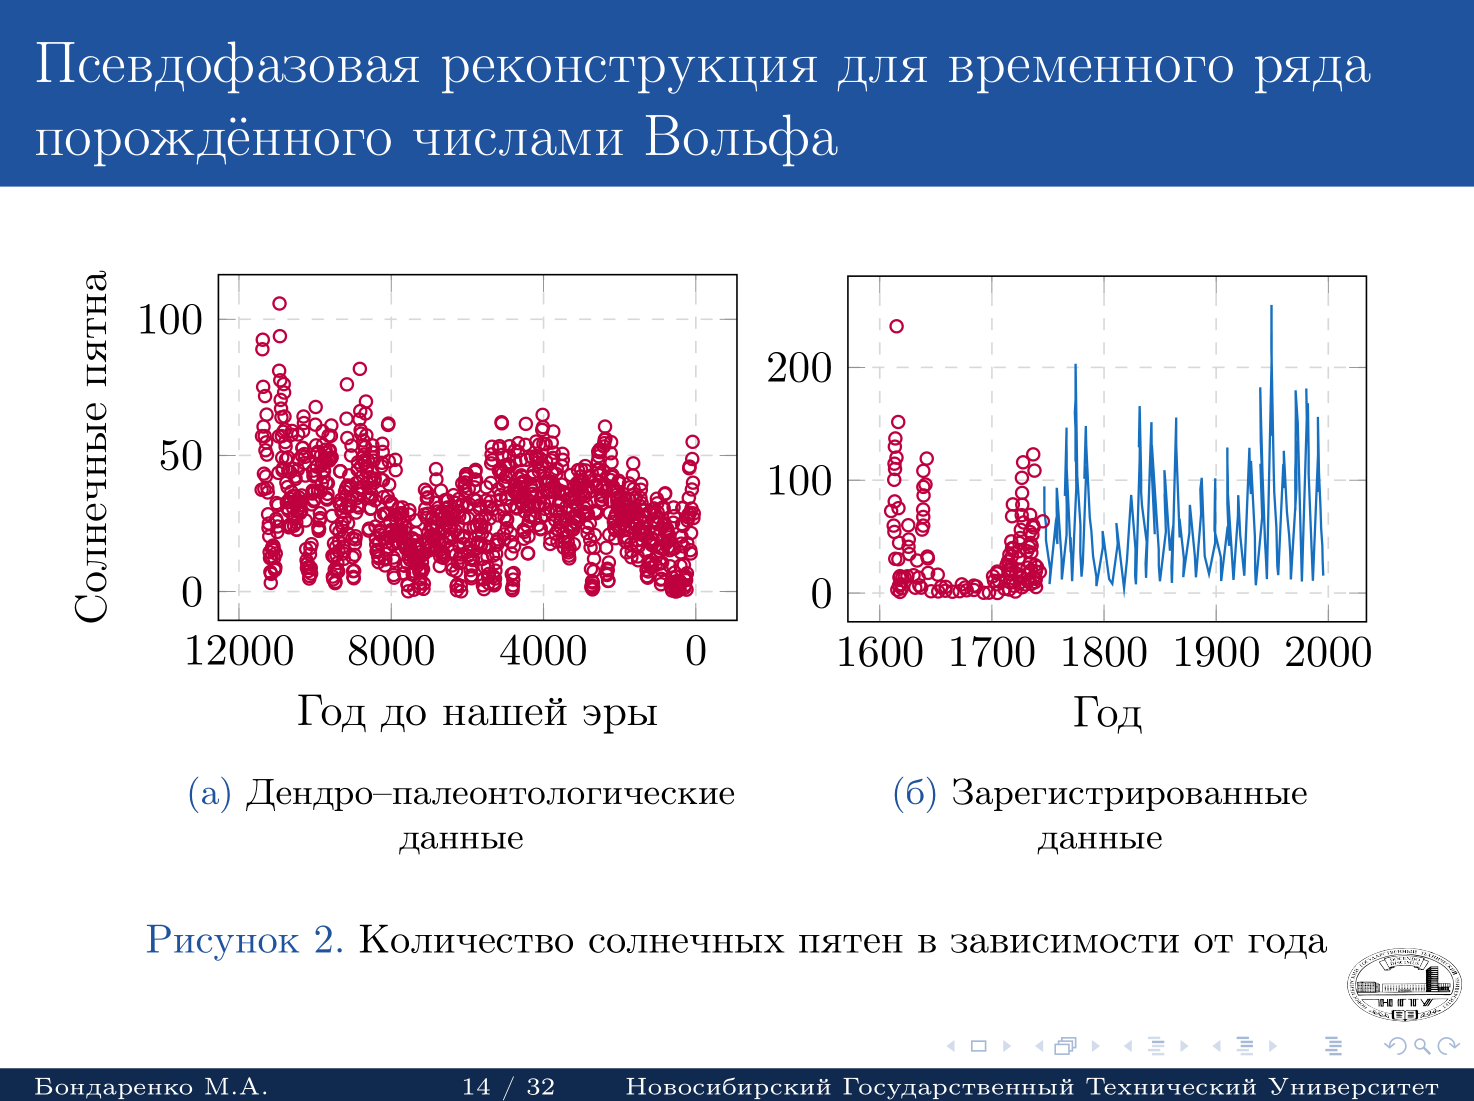
\includegraphics[width=.8\textwidth]{pics/present-graphs.png}}
\caption{Пример слайда с графиками.}
\label{pic-pres-graph}
\end{figure}
\begin{figure}[H]
\fboxsep=0mm
\centering
\fbox{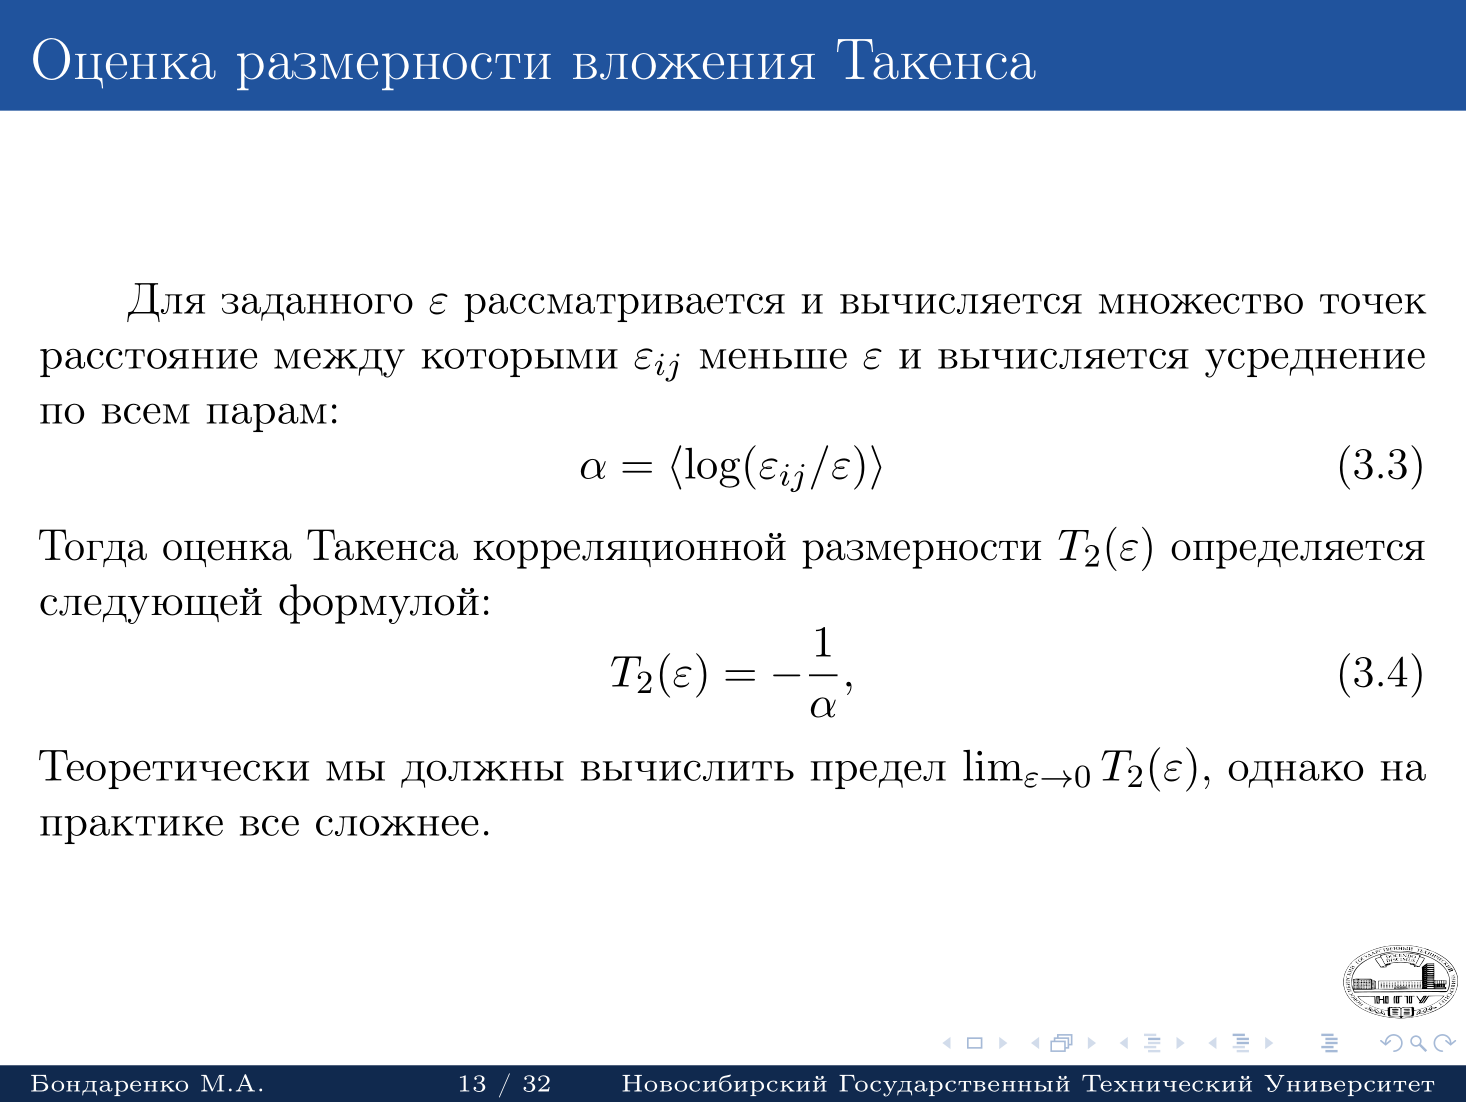
\includegraphics[width=.8\textwidth]{pics/present-formula.png}}
\caption{Пример слайда с формулами.}
\label{pic-pres-formula}
\end{figure}









%\backmatter %% это выключает нумерацию для Заключения и Списка литературы

%\input{ending.tex} 

\clearpage

\setcounter{biburllcpenalty}{7000}
\setcounter{biburlucpenalty}{8000}

\phantomsection
\addcontentsline{toc}{section}{Список использованных источников}
\section*{Список использованных источников}
\defbibheading{bibliography}{}%\Large\bf Список использованных источников}
\printbibliography


%\clearpage
\ifdefmacro{\microtypesetup}{\microtypesetup{protrusion=false}}{} % не рекомендуется применять пакет микротипографики к автоматически генерируемым спискам
\phantomsection
\listoffigures  % Список изображений

%%% Список таблиц %%%
% (ГОСТ Р 7.0.11-2011, 5.3.10)
\clearpage
\phantomsection
\listoftables   % Список таблиц
\ifdefmacro{\microtypesetup}{\microtypesetup{protrusion=true}}{}
\newpage

\clearpage

%\input{appendix}
%\listoftodos
\end{document}






